% Copyright (c) 2014 Jeremie DECOCK (http://www.jdhp.org)

\documentclass{article}

\usepackage[utf8]{inputenc}
\usepackage[T1]{fontenc}

% English environment
%\usepackage[english]{babel}

% French environment
%\usepackage[french]{babel}

% French + English environment
%\usepackage[francais,english]{babel}

%%%%%%%%%%%%%%%%%%%%%%%%%%%%%%%%%%%%%%%%%%%%%%%%%%%%%%%%%%%%%%%%%%%%%%%%%%%%%%%%

% Clickable Table of Contents
% http://tex.stackexchange.com/questions/73862/how-can-i-make-a-clickable-table-of-contents
\usepackage{hyperref}
\hypersetup{
	pdftoolbar=true,                                          % show Acrobat’s toolbar ?
	pdfmenubar=true,                                          % show Acrobat’s menu ?
	pdffitwindow=true,                                        % page fit to window when opened
	pdfnewwindow=true,                                        % links in new window
	colorlinks=true,                                          % false: boxed links; true: colored links
	linkcolor=black,                                          % color of internal links
	citecolor=black,                                          % color of links to bibliography
	filecolor=black,                                          % color of file links
	urlcolor=black                                            % color of external links
}

\usepackage{algorithm}
\usepackage{algorithmic}
\usepackage{amsmath}
\usepackage{amssymb}
%\usepackage{bm}    % bold math
\usepackage{color}  % change text color
\usepackage{xcolor} % required for listings package...
\usepackage{epsfig}
\usepackage{eurosym}
\usepackage{flushend}
\usepackage{graphicx}
\usepackage{ifthen}
\usepackage{multirow}
%\usepackage{natbib} % For bibliography, often used nowadays
\usepackage{subfigure}
\usepackage{url}

%% Inserting a pdf file in the document
%% See: http://stackoverflow.com/questions/2739159/inserting-a-pdf-file-in-latex 
%\usepackage{pdfpages}
%\usepackage{epsfig}
%\usepackage{geometry}
%\usepackage{pdflscape}

%%%%%%%%%%%%%%%%%%%%%%%%%%%%%%%%%%%%%%%%%%%%%%%%%%%%%%%%%%%%%%%%%%%%%%%%%%%%%%%%

%\usepackage[font=sf, labelfont={sf,bf}, margin=1cm]{caption}
%\usepackage[font=rm, margin=1cm]{caption}

% HeVeA %%%%%%%%%%%%%%%%%%%%%%%%%%%%%%%%%%%%%%%%%%%%%%%%%%%%%%%%%%%%%%%%%%%%%%%

\usepackage{hevea}
\newstyle{body}{margin-left: auto; margin-right: auto; padding: .5em 1.5em; max-width: 50em; text-align: justify; font-family: sans-serif;}
\newstyle{div.lstlisting}{font-size: 130\%; margin-left: auto; margin-right: auto; width: 35em;}

\newif\ifpdf                   
\ifx\pdfoutput\undefined
\pdffalse
\else
\pdfoutput=1
\pdftrue
\fi

% TikZ %%%%%%%%%%%%%%%%%%%%%%%%%%%%%%%%%%%%%%%%%%%%%%%%%%%%%%%%%%%%%%%%%%%%%%%%

%\usepackage{tikz}
%\usetikzlibrary{matrix} % for block alignment
\usetikzlibrary{arrows} % for arrow heads
\usetikzlibrary{calc}   % for manipulation of coordinates
\usetikzlibrary{positioning} 
\usetikzlibrary{patterns}



% Listings package settings %%%%%%%%%%%%%%%%%%%%%%%%%%%%%%%%%%%%%%%%%%%%%%%%%%%%

\usepackage{listings}

% Listings package settings %%%%%%%%%%%%%%%%%%%%%%%%%%%%%%%%%%%%%%%%%%%%%%%%%%%%

% See http://en.wikibooks.org/wiki/LaTeX/Source_Code_Listings

% By default, listings does not support multi-byte encoding for source code. The extendedchar option only works for 8-bits encodings such as latin1.
% To handle UTF-8, you should tell listings how to interpret the special characters by defining them like so
\lstset{literate=
    {á}{{\'a}}1 {é}{{\'e}}1 {í}{{\'i}}1 {ó}{{\'o}}1 {ú}{{\'u}}1
    {Á}{{\'A}}1 {É}{{\'E}}1 {Í}{{\'I}}1 {Ó}{{\'O}}1 {Ú}{{\'U}}1
    {à}{{\`a}}1 {è}{{\'e}}1 {ì}{{\`i}}1 {ò}{{\`o}}1 {ù}{{\`u}}1
    {À}{{\`A}}1 {È}{{\'E}}1 {Ì}{{\`I}}1 {Ò}{{\`O}}1 {Ù}{{\`U}}1
    {ä}{{\"a}}1 {ë}{{\"e}}1 {ï}{{\"i}}1 {ö}{{\"o}}1 {ü}{{\"u}}1
    {Ä}{{\"A}}1 {Ë}{{\"E}}1 {Ï}{{\"I}}1 {Ö}{{\"O}}1 {Ü}{{\"U}}1
    {â}{{\^a}}1 {ê}{{\^e}}1 {î}{{\^i}}1 {ô}{{\^o}}1 {û}{{\^u}}1
    {Â}{{\^A}}1 {Ê}{{\^E}}1 {Î}{{\^I}}1 {Ô}{{\^O}}1 {Û}{{\^U}}1
    {œ}{{\oe}}1 {Œ}{{\OE}}1 {æ}{{\ae}}1 {Æ}{{\AE}}1 {ß}{{\ss}}1
    {ç}{{\c c}}1 {Ç}{{\c C}}1 {ø}{{\o}}1 {å}{{\r a}}1 {Å}{{\r A}}1
    {€}{{\EUR}}1 {£}{{\pounds}}1
}

\usepackage{color}

\definecolor{mygreen}{rgb}{0,0.6,0}
\definecolor{mygray}{rgb}{0.5,0.5,0.5}
\definecolor{mymauve}{rgb}{0.58,0,0.82}

\lstset{ %
  backgroundcolor=\color{white},   % choose the background color; you must add \usepackage{color} or \usepackage{xcolor}
  basicstyle=\footnotesize,        % the size of the fonts that are used for the code
  breakatwhitespace=false,         % sets if automatic breaks should only happen at whitespace
  breaklines=true,                 % sets automatic line breaking
  captionpos=b,                    % sets the caption-position to bottom
  commentstyle=\color{mygreen},    % comment style
  deletekeywords={...},            % if you want to delete keywords from the given language
  escapeinside={\%*}{*)},          % if you want to add LaTeX within your code
  extendedchars=true,              % lets you use non-ASCII characters; for 8-bits encodings only, does not work with UTF-8
  frame=L,                    % adds a frame around the code
  keepspaces=true,                 % keeps spaces in text, useful for keeping indentation of code (possibly needs columns=flexible)
  keywordstyle=\color{blue},       % keyword style
  %language=Octave,                % the language of the code
  morekeywords={*,...},            % if you want to add more keywords to the set
  numbers=left,                    % where to put the line-numbers; possible values are (none, left, right)
  numbersep=10pt,                  % how far the line-numbers are from the code
  numberstyle=\tiny\color{mygray}, % the style that is used for the line-numbers
  rulecolor=\color{black},         % if not set, the frame-color may be changed on line-breaks within not-black text (e.g. comments (green here))
  showspaces=false,                % show spaces everywhere adding particular underscores; it overrides 'showstringspaces'
  showstringspaces=false,          % underline spaces within strings only
  showtabs=false,                  % show tabs within strings adding particular underscores
  stepnumber=1,                    % the step between two line-numbers. If it's 1, each line will be numbered
  stringstyle=\color{mymauve},     % string literal style
  tabsize=2,                       % sets default tabsize to 2 spaces
  title=\lstname                   % show the filename of files included with \lstinputlisting; also try caption instead of title
}

\lstdefinestyle{customc}{
  belowcaptionskip=1\baselineskip,
  breaklines=true,
  frame=L,
  xleftmargin=\parindent,
  language=C,
  showstringspaces=false,
  basicstyle=\footnotesize\ttfamily,
  keywordstyle=\bfseries\color{green!40!black},
  commentstyle=\itshape\color{purple!40!black},
  identifierstyle=\color{blue},
  stringstyle=\color{orange},
}

\lstdefinestyle{customasm}{
  belowcaptionskip=1\baselineskip,
  frame=L,
  xleftmargin=\parindent,
  language=[x86masm]Assembler,
  basicstyle=\footnotesize\ttfamily,
  commentstyle=\itshape\color{purple!40!black},
}

\lstset{escapechar=@,style=customc}



%% COMMANDS AND DEFS %%%%%%%%%%%%%%%%%%%%%%%%%%%%%%%%%%%%%%%%%%%%%%%%%%%%%%%%%%%

% Pour désactiver temporairement les images (compile beaucoup plus vite)
%\renewcommand{\includegraphics}[2][]{\null}

%%% Math symbols

%\renewcommand{\vec}[1]{\ensuremath{\boldsymbol{#1}}} % bold vectors
\newcommand{\vs}[1]{\boldsymbol{#1}} % vector symbol (\boldsymbol, \textbf or \vec)
\newcommand{\ms}[1]{\boldsymbol{#1}} % matrix symbol (\boldsymbol, \textbf)

\newcommand{\x}{\vs{x}}
\newcommand{\xstar}{\vs{x^*}}
\newcommand{\w}{\vs{\omega}}
\newcommand{\objfunc}{f}

\def\bbbr{{\rm I\!R}} % reelle Zahlen

\newcommand{\E}{\mathbb{E}}
\newcommand{\N}{\mathbb{N}}
\newcommand{\Z}{\mathbb{Z}}
\newcommand{\Q}{\mathbb{Q}}
\newcommand{\R}{{\bbbr}{}}
\newcommand{\C}{\mathbb{C}}
\newcommand{\K}{\mathbb{K}}

\newcommand{\mb}[1]{\mathbb{#1}}
\newcommand{\mc}[1]{\mathcal{#1}}

\def\CQFD{\fbox\\}

%%% General commands

\newenvironment{jmatrix}{\renewcommand\arraystretch{1.5} \begin{pmatrix}}{\end{pmatrix}}
%\renewcommand{\arraystretch}{1.5}

\newcommand{\cred}[1]{\textcolor{red}{#1}}
\newcommand{\ech}[1]{\textcolor{gray}{#1}}
\newcommand{\imp}[1]{{\em {#1}}}
\newcommand{\voc}[1]{{\em {#1}}}
\newcommand{\todo}[1][\dots]{\textbf{[TODO : #1]}}  % todo mark

\newcommand{\dontforget}[1]{\textcolor{red}{#1}}

\newcommand{\HRule}{\rule{\linewidth}{0.5mm}}

%%% Debug: Display the current table counter (cf. http://www.iam.ubc.ca/old_pages/newbury/tex/numbering.html)

\newcommand{\tablecounterdebug}{\textbf{Table~counter:~\thetable}\\}
\newcommand{\equationcounterdebug}{\textbf{Equation~counter:~\theequation}\\}
\newcommand{\figurecounterdebug}{\textbf{Figure~counter:~\thefigure}\\}
\newcommand{\algorithmcounterdebug}{\textbf{Algorithm~counter:~\thealgorithm}\\}



\sloppy

%%%%%%%%%%%%%%%%%%%%%%%%%%%%%%%%%%%%%%%%%%%%%%%%%%%%%%%%%%%%%%%%%%%%%%%%%%%%%%%

\title{Put a title here}

\author{Jérémie \textsc{Decock} \\ \url{http://www.jdhp.org}}

%\institute{ \textsuperscript{1}TAO, INRIA-CNRS-LRI, Univ. Paris-Sud, 91190 Gif-sur-Yvette, France}

\hypersetup{
	pdftitle={Put a title here},     % title
	pdfauthor={Jérémie DECOCK},      % author
	pdfsubject={Put a subject here}, % subject of the document
	pdfkeywords={key, words}         % list of keywords
}

%%%%%%%%%%%%%%%%%%%%%%%%%%%%%%%%%%%%%%%%%%%%%%%%%%%%%%%%%%%%%%%%%%%%%%%%%%%%%%%

\begin{document}

\maketitle

\begin{abstract}
  Blablabla
\end{abstract}

\tableofcontents

% Introduction %%%%%%%%%%%%%%%%%%%%%%%%%%%%%%%%%%%%%%%%%%%%%%%%%%%%%%%%%%%%%%%%

\section*{Introduction}\label{sec:intro}

% Section 1 %%%%%%%%%%%%%%%%%%%%%%%%%%%%%%%%%%%%%%%%%%%%%%%%%%%%%%%%%%%%%%%%%%%

\section{Test}\label{sec:test}

Blablabla \cite{decock:hal-00755663}.

% Section 2 %%%%%%%%%%%%%%%%%%%%%%%%%%%%%%%%%%%%%%%%%%%%%%%%%%%%%%%%%%%%%%%%%%%

\section{Snippets}\label{sec:snippets}

\subsection{Lists}\label{subsec:lists}

\begin{itemize}
    \item item 1
    \item item 2
    \item \dots
\end{itemize}

\begin{enumerate}
    \item item 1
    \item item 2
    \item \dots
\end{enumerate}

\begin{description}
    \item[First] item 1
    \item[Second] item 2
    \item[Last] \dots
\end{description}


\subsection{Sizes}\label{subsec:sizes}

\begin{small}
small
\end{small}

\begin{footnotesize}
footnotesize
\end{footnotesize}

\begin{scriptsize}
scriptsize
\end{scriptsize}

\begin{tiny}
tiny
\end{tiny}


\subsection{Colors}\label{subsec:colors}

{\color{red} Red}
{\color{green} Green}
{\color{blue} Blue}


\subsection{Image}\label{subsec:image}

\begin{figure}
    \centering
    \ifpdf
    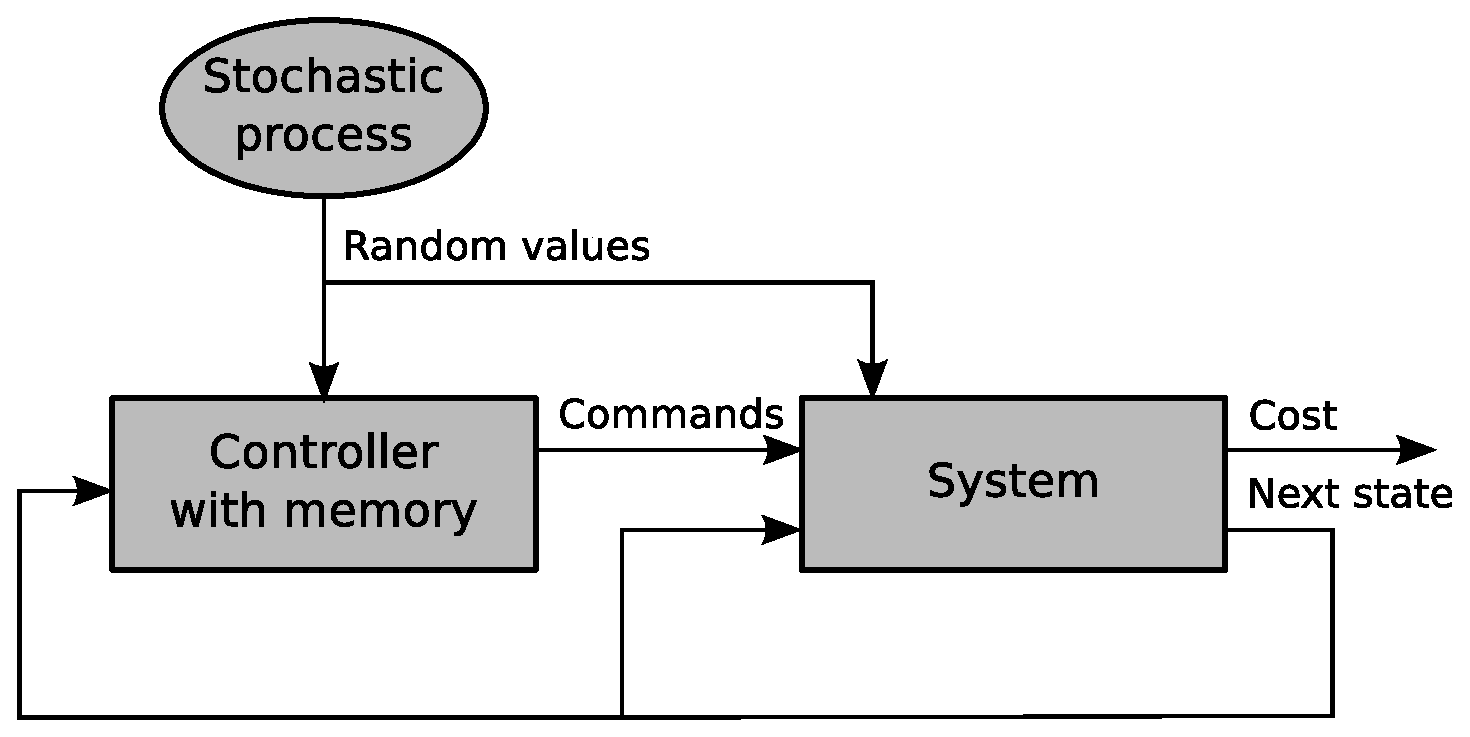
\includegraphics[width=.80\linewidth]{fig/test.pdf}
    \else
    \imgsrc{fig/test.png}
    \fi
    \caption{\label{fig:test}Test}
\end{figure}


\subsection{Subfigures}\label{subsec:subfig}

\begin{figure}
    \centering
    \subfigure{
        \ifpdf
        
\includegraphics[width=.30\linewidth,height=.20\linewidth]{fig/test}
        \else
        \imgsrc{fig/test.png}
        \fi
    }~
    \subfigure{
        \ifpdf
        
\includegraphics[width=.30\linewidth,height=.20\linewidth]{fig/test}
        \else
        \imgsrc{fig/test.png}
        \fi
    }~
    \subfigure{
        \ifpdf
        
\includegraphics[width=.30\linewidth,height=.20\linewidth]{fig/test}
        \else
        \imgsrc{fig/test.png}
        \fi
    }
    ~\\
    \subfigure{
        \ifpdf
        
\includegraphics[width=.30\linewidth,height=.20\linewidth]{fig/test}
        \else
        \imgsrc{fig/test.png}
        \fi
    }~
    \subfigure{
        \ifpdf
        
\includegraphics[width=.30\linewidth,height=.20\linewidth]{fig/test}
        \else
        \imgsrc{fig/test.png}
        \fi
    }~
    \subfigure{
        \ifpdf
        
\includegraphics[width=.30\linewidth,height=.20\linewidth]{fig/test}
        \else
        \imgsrc{fig/test.png}
        \fi
    }
\end{figure}


\subsection{Equations}\label{subsec:eq}

$$
    V(x) = \max_{a \in \Gamma (x) } \{ F(x,a) + \beta V(T(x,a)) \}  \label{eq:bellman}
$$

\[
    V(x) = \max_{a \in \Gamma (x) } \{ F(x,a) + \beta V(T(x,a)) \}  \label{eq:bellman}
\]

\begin{equation}
    V(x) = \max_{a \in \Gamma (x) } \{ F(x,a) + \beta V(T(x,a)) \}  \label{eq:bellman}
\end{equation}


\subsection{Equation array}\label{subsec:eqarray}

\begin{eqnarray*}
    \mbox{Expectation of N} & = & \sum_{i=1}^{n} \E(Z_i) \\
                            & = & \sum_{i=1}^{n} \frac{\gamma}{d^{\beta/2}} \frac{ c(d)^\beta }{i^{\alpha\beta}} \\
                            & = & \frac{\gamma}{d^{\beta/2}} c(d)^\beta \sum_{i=1}^{n} \frac{1}{i^{\alpha\beta}} \\
                            & = & z \\
                            & ~ & \\
\end{eqnarray*}
\begin{eqnarray}
    \mbox{Variance of N} & = & \sum_{i=1}^{n} V(Z_i) \\
                         & \leq & \sum_{i=1}^{n} \E(Z_i) ~~~~~~~ (\mbox{as } V(Z_i) \leq \E(Z_i)) \\
                         & \leq & z  \nonumber
\end{eqnarray}


\subsection{Matrices}\label{subsec:matrices}

$$
    A_{m,n} =
    \begin{pmatrix}
        a_{1,1} & a_{1,2} & \cdots & a_{1,n} \\
        a_{2,1} & a_{2,2} & \cdots & a_{2,n} \\
        \vdots  & \vdots  & \ddots & \vdots  \\
        a_{m,1} & a_{m,2} & \cdots & a_{m,n}
    \end{pmatrix}
$$

$$
    M =
    \begin{bmatrix}
        \frac{5}{6} & \frac{1}{6} & 0           \\[0.3em]
        \frac{5}{6} & 0           & \frac{1}{6} \\[0.3em]
        0           & \frac{5}{6} & \frac{1}{6}
    \end{bmatrix}
$$

$$
    M = \bordermatrix{~ & x & y \cr
                      A & 1 & 0 \cr
                      B & 0 & 1 \cr}
$$


\subsection{Systems of equation array}\label{subsec:syseq}

\[
    f(n) = \left\{
    \begin{array}{l l}
        n/2      & \quad \text{if $n$ is even}\\
        -(n+1)/2 & \quad \text{if $n$ is odd}
    \end{array} \right.
\]


\subsection{Mathematical programming}\label{subsec:mathprog}

\begin{align}
    \max        & \quad z = 4 x_1 + 7 x_2    \notag \\
    \text{s.t.} & \quad 3 x_1 + 5 x_2 \leq 6 \label{constraint1}\\
                & \quad   x_1 + 2 x_2 \leq 8 \label{constraint2}\\
                & \quad   x_1, x_2 \geq 0    \notag
\end{align}


% see http://tex.stackexchange.com/questions/75108/how-to-edit-the-linear-programming-in-latex
% and http://tex.stackexchange.com/questions/83918/labeled-linear-program-with-labeled-equations-and-wide-objective-function

% see http://latex.wikia.com/wiki/List_of_LaTeX_environments for explanations about alignat

% The alignat environment can be used to align equations, and explicitly
% specify the number of "equation" columns. An equation column has two
% parts, separated by the equals-sign. Essentially, this is an array with
% alternating right-aligned and left-aligned columns. The required
% parameter of alignat is the maximum number of ampersands in a row plus 1,
% and then divided by 2. One use of alignat is to explicitly specify the
% amount of horizontal space between columns by including the required
% spacing in the first row.

% \rlap is used since the operators in the first equation have no business
% being aligned with the rest.

%    %\begin{alignat*}{6}   % argument = at least (the number of '&' + 1) / 2
%    %    \text{Max}  \quad \rlap{$z = x_1 + 12x_2$}                                       \\               
%    %    \text{s.t.} \quad & 13 & x_1 & {}+{} &  & x_2 & {}+{} & 12 & x_3 & ~ \leq ~ & 5  \\
%    %                      &    & x_1 &       &  &     & {}+{} &    & x_3 & ~ \leq ~ & 16 \\
%    %                      & 15 & x_1 & {}+{} &  & x_2 &       &    &     & ~ =    ~ & 14 \\
%    %                      & \rlap{$x_j \geqslant 0,\; j=1,2,3.$}
%    %\end{alignat*}
%
%    \begin{alignat*}{5}  % argument = at least (the number of '&' + 1) / 2
%        \text{Max}  \quad \rlap{$z = x_1 + 12x_2$}                                   \\               
%        \text{s.t.} \quad & & 13 x_1 & {}+{} &  x_2 & {}+{} & 12 x_3 & ~ \leq ~ & 5  \\
%                          & &    x_1 &       &      & {}+{} &    x_3 & ~ \leq ~ & 16 \\
%                          & & 15 x_1 & {}+{} &  x_2 &       &        & ~ =    ~ & 14 \\
%                          & \rlap{$x_j \geq 0, ~ j=1,2,3.$}
%    \end{alignat*}
%
%    \begin{alignat}{5}   % argument = at least (the number of '&' + 1) / 2
%        \text{Max}  \quad \rlap{$z = x_1 + 12x_2$}                                  \nonumber  \\
%        \text{s.t.} \quad & & 13 x_1 & {}+{} & x_2 & {}+{} & 12 x_3 & ~ \leq ~ & 5  \label{c1} \\
%                          & &    x_1 &       &     & {}+{} &    x_3 & ~ \leq ~ & 16 \label{c2} \\
%                          & & 15 x_1 & {}+{} & x_2 &       &        & ~ =    ~ & 14 \label{c3} \\
%                          & \rlap{$x_j \geq 0, ~ j=1,2,3.$}                         \nonumber
%    \end{alignat}


\subsection{Algorithms}\label{subsec:algorithms}
% Algorithmic commands:
%  \STATE <text>
%  \IF{<condition>} \STATE{<text>} \ENDIF
%  \FOR{<condition>} \STATE{<text>} \ENDFOR
%  \FOR{<condition> \TO <condition> } \STATE{<text>} \ENDFOR
%  \FORALL{<condition>} \STATE{<text>} \ENDFOR
%  \WHILE{<condition>} \STATE{<text>} \ENDWHILE
%  \REPEAT \STATE{<text>} \UNTIL{<condition>}
%  \LOOP \STATE{<text>} \ENDLOOP
%  \REQUIRE <text>
%  \ENSURE <text>
%  \RETURN <text>
%  \PRINT <text>
%  \COMMENT{<text>}
%  \AND, \OR, \XOR, \NOT, \TO, \TRUE, \FALSE
\begin{algorithmic}
    \REQUIRE ~\\
             $\langle \mathcal{S}, \mathcal{A}, T, R \rangle$, an MDP\\
             $\gamma$, the discount factor\\
             $\epsilon$, the maximum error allowed in the utility of any state in an iteration
    %\ENSURE ~\\
    %        $U, U'$, vector of utilities for states in $\mathcal{S}$, initially zero\\
    %        $\delta$, the maximum change in the utility of any state in an iteration\\
    \STATE \hspace{-1em}\textbf{Local variables:}\\
            $U, U'$, vector of utilities for states in $\mathcal{S}$, initially zero\\
            $\delta$, the maximum change in the utility of any state in an iteration\\
            ~

    \REPEAT
        \STATE $U \leftarrow U'$
        \STATE $\delta \leftarrow 0$
        \FORALL{$s \in \mathcal{S}$}
            \STATE $U'[s] \leftarrow R[s] + \gamma \max_a \sum_{s'} T(s,a,s') U[s']$
            \IF{$|U'[s] - U[s]| > \delta$}
                \STATE $\delta \leftarrow |U'[s] - U[s]|$
            \ENDIF
        \ENDFOR
    \UNTIL{$\delta < \epsilon(1-\gamma)/\gamma$}
    ~

    \RETURN $U$
\end{algorithmic}


\subsection{Listings}\label{subsec:listings}

\begin{small}
    \lstinputlisting[language=Python]{listings/test.py}
    %\lstinputlisting[language=Python, firstline=2, lastline=5]{listings/test.py}
\end{small}


\subsection{Verbatim}\label{subsec:verbatim}

\begin{verbatim}
    .--.
   |o_o |
   |:_/ |
  //   \ \
 (|     | )
/'\_   _/`\
\___)=(___/

# gcc -o hello hello.c
\end{verbatim}


\subsection{Table}\label{subsec:table}

\begin{tabular}{|l|c|c|}
\hline
                          & $\gamma=1$ (small noise)                      & $\gamma<1$ (large noise) \\
\hline
Proved rate for R-EDA     & $\frac{1}{\beta} \leq {\color{blue} \alpha}$  & $\frac{1}{2\beta} \leq {\color{blue} \alpha}$ \\
\hline
Former lower bounds       & ${\color{blue} \alpha} \leq 1$                & ${\color{blue} \alpha} \leq 1$ \\
\hline
R-EDA experimental rates  & ${\color{blue} \alpha} = \frac{1}{\beta}$     & ${\color{blue} \alpha} = \frac{1}{2\beta}$ \\
\hline
\hline
Rate by active learning   & ${\color{blue} \alpha} = \frac{1}{2}$        & ${\color{blue} \alpha} = \frac{1}{2}$   \\
\hline
\end{tabular}


\subsection{URL}\label{subsec:url}

\url{http://www.jdhp.org/}  \\
\href{http://www.jdhp.org/}{JDHP}

% Section CCL %%%%%%%%%%%%%%%%%%%%%%%%%%%%%%%%%%%%%%%%%%%%%%%%%%%%%%%%%%%%%%%%%

\section*{Conclusion}\label{sec:ccl}
 
...

% Section License %%%%%%%%%%%%%%%%%%%%%%%%%%%%%%%%%%%%%%%%%%%%%%%%%%%%%%%%%%%%%

\section*{License}\label{sec:license}
 
...
% HeVeA
\begin{rawhtml}

    <div>
        <a rel="license" href="http://creativecommons.org/licenses/by-sa/4.0/">
            <img alt="Licence Creative Commons" style="border-width:0" src="https://i.creativecommons.org/l/by-sa/4.0/80x15.png" />
        </a>
        <br />
        <span xmlns:dct="http://purl.org/dc/terms/" href="http://purl.org/dc/dcmitype/Text" property="dct:title" rel="dct:type">Title...</span> de <a xmlns:cc="http://creativecommons.org/ns#" href="http://www.jdhp.org" property="cc:attributionName" rel="cc:attributionURL">Jérémie Decock</a> est mis à disposition selon les termes de la <a rel="license" href="http://creativecommons.org/licenses/by-sa/4.0/">licence Creative Commons Attribution -  Partage dans les Mêmes Conditions 4.0 International</a>.
    </div>

\end{rawhtml}

% Bibliography %%%%%%%%%%%%%%%%%%%%%%%%%%%%%%%%%%%%%%%%%%%%%%%%%%%%%%%%%%%%%%%%

%\nocite{decock:hal-00755663}  % fait apparaitre le document dans la bibliographie sans le citer !
%\nocite{*}                    % fait apparaitre TOUS les documents du .bib dans la bibliographie sans les citer !

\bibliographystyle{plain}    % name of the .bst file (bibliography style)
\bibliography{bibliography}  % name of the .bib file (without the file name extension)

\end{document}

